\chapter{Cloud macrophysical and radiative properties observed during the Norwegian Young Sea Ice field campaign}
\vspace{1 cm}
\begin{spacing}{1} \begin{quote} 
\noindent \emph{The combined effect of all climate feedback processes is to amplify the climate response to forcing (virtually certain). While major advances in the understanding of cloud processes have increased the level of confidence and decreased the uncertainty range for the cloud feedback by about 50 $\%$ compared to AR5, clouds remain the largest contribution to overall uncertainty in climate feedbacks (high confidence).} \end{quote}
\hspace{6 cm} - IPCC Sixth Assessment Report, August 2021  
\end{spacing}
\vspace{1 cm}
\noindent Sarah Y. Murphy$^1$, Von P. Walden$^1$, Stephen R. Hudson$^2$, Lana Cohen$^2$, and Robert Stillwell$^3$ 


\noindent $^1$Washington State University, Pullman, Washington, USA\\
$^2$Norwegian Polar Institute, Fram Centre, Tromsø, Norway\\
$^3$National Center for Atmospheric Research, Boulder, Colorado, USA\\

\begin{center}
    \emph{Publication in preparation}
\end{center}

\section{Introduction}

The global climate is heavily influenced by processes that occur in the Arctic. However, the Arctic environment is currently experiencing rapid change \citep{overland:2011, stroeve:2007}. Due to a lack of observations, it has been difficult to fully understand atmospheric processes in the polar regions \citep{persson:2002}. The atmospheric circulation in the Arctic is modified by changes in the overall climate, which, in turn, impact cloudiness and radiation at the surface \citep{zhang:2008}. The Advanced Very High-Resolution Radiometer has observed that wintertime cloud cover over the Arctic Ocean is decreasing by 5 $\%$ per decade. Meanwhile, in spring, increases as large as 15 $\%$ per decade have been observed, which can likely be attributed to changes in atmospheric circulation \citep{schweiger:2004}. A decreasing trend in Arctic sea ice of -2.9 $\%$ to -9.1 $\%$ per decade was seen from 1979 through 2006 \citep{stroeve:2007}. Measurements of the energy balance and cloud properties (fraction, height, microphysical, and temperature) can give important insight into climate processes and radiative transfer but are rarely measured together \citep{persson:2002, schweiger:2004, miller:2017}. 

The Norwegian Young Sea Ice Experiment (N-ICE2015, or N-ICE) \citep{granskog:2018} is the first experiment to make comprehensive measurements of clouds and the surface energy balance from winter to summer since the Surface Heat Budget of the Arctic Ocean Experiment (SHEBA) in 1997 and 1998 \citep{walden:2017, uttal:2002}. SHEBA took place north of Alaska in the Beaufort and Chukchi Seas, while N-ICE was conducted north of Svalbard in the Arctic Ocean, measuring the components surface energy budget \citep{persson:2002, andreas:2010, grachev:2007}, cloud properties \citep{turner:2005, turner:2002, intrieri:2002, shupe:2004}, and the resulting surface properties \citep{intrieri:2002, shupe:2004}. Other experiments since SHEBA, such as the Arctic Ocean Experiment (AOE-2001) \citep{tjernstrom:2005}, Atmospheric Conditions during the Arctic Clouds in Summer Experiment (ACSE) \citep{sotiropoulou:2016}, and the Mixed-Phase Arctic Cloud Experiment \citep{verlinde:2007} have not observed winter or took place over a shorter duration than N-ICE. Prior to SHEBA, field experiments such as the Seasonal Ice Zone Experiment, Coordinated Eastern Arctic experiment, Marginal Ice Zone Experiments, Arctic Ice Dynamics Joint Experiment, and Soviet drifting stations \citep{vihma:2005, kahl:1999} that collected meteorological and radiation data over Arctic sea ice either covered a small area or had poor temporal resolution. However, these studies have used observations of cloud cover, albedo, and cloud properties to provide estimates of the surface energy budget. Comparing SHEBA data to these estimates showed that during transition seasons (September, October, November, March, and April), the SHEBA time period had larger incoming longwave radiation and a smaller magnitude of shortwave radiation, sensible heat flux, and latent heat flux compared to other studies. This could be caused by a higher frequency of warm air masses, an increase in cloud cover, or a combination of both \citep{persson:2002}. 

SHEBA was conducted almost two decades before N-ICE. Measurements were taken further into the ice pack \citep{cohen:2017} and in thicker ice conditions. In addition, the meteorological conditions were different; detailed comparisons of N-ICE and SHEBA during the winter can be found in \citep{graham:2017}. There were a few warm events during N-ICE caused by synoptic storms when temperatures reach 0 $^{\circ} C$; these events were much warmer than any of the warm periods experienced during SHEBA. In addition, the near-surface temperatures were more variable during N-ICE \citep{cohen:2017}. During the warm periods at N-ICE, the cloud properties were quite variable, suggesting that some of the changes in the surface energy balance could be the result of changes in cloud macrophysical and/or microphysical properties. Throughout SHEBA, mixed-phase clouds were observed 41 $\%$ of the time. \citet{graham:2017} states that in the winter, radiative cooling events were more frequent during the N-ICE period than during SHEBA. 

Due to their importance to the surface energy budget over the Arctic Ocean, it is important to investigate the properties and radiative forcing of clouds during N-ICE and to compare the results to those observed during SHEBA. These results will provide useful constraints for models that traditionally have had difficulty simulating radiation at the surface of Arctic sea ice. Proper modeling of Arctic clouds in all seasons is essential for simulating accurate values of the surface energy budget, which is critical for modeling the seasonal cycle of sea ice. A critical parameter that was identified during SHEBA \citep{inoue:2008, tjernstrom:2005} and other Arctic field experiments \citep{hines:2017, listowski:2017, hines:2019}.is the fraction of mixed-phase clouds. \citet{graham:2017} showed that six atmospheric reanalyses have difficulty simulating Arctic clouds.

This paper uses various observations obtained during the N-ICE2015 field campaign to document the cloud macrophysical properties, the shortwave (SW) and longwave (LW) radiation, and the net cloud radiative forcing (CRF) at the surface of young Arctic sea ice. Section 2 describes the various measurements that were made during N-ICE to estimate CRF. Section 3 describes the methods to calculate CRF, which involved combining N-ICE measurements with radiative transfer modeling. Section 4 describes the seasonal transition of CRF from winter to summer. Section 5 presents the conclusions of this study.


\section{Measurements}

The Norwegian Young Sea Ice Experiment (N-ICE) was conducted during the six-month transition from winter to summer (January - June 2015) in the Arctic Ocean north of Svalbard. All of the instruments were either deployed onboard the Norwegian research vessel Lance or on the sea ice near the Lance. The instruments used in this study were a Vaisala CL-25 ceilometer, a Micropulse Lidar (MPL), twice-daily Vaisala radiosondes, and Kipp and Zonen shortwave and longwave broadband radiometers. This field campaign was the first since SHEBA to make detailed atmospheric and cloud observations during the winter-to-summer transition in the Arctic. More information about N-ICE can be found in Chapter 2. 

The synoptic context of the N-ICE field campaign is described by \citet{cohen:2017}. The storms designated in Table 2 of \citet{cohen:2017} are of particular interest to this study. Six major and three minor storms occurred in winter (between 21 January and 14 March), while two major and seven minor storms occur in spring and summer (from 23 April through 11 June). The winter was characterized by a succession of particularly strong storms (as compared to climatology), while the spring conditions were typical of that region of the Arctic \citep{graham:2017}. The winter storms were accompanied by large increases in the integrated water vapor and changes in wind direction \citep{kayser:2017} that influenced cloud properties.  

A list of the meteorological instrumentation deployed during N-ICE is given in Table 1 of \citet{cohen:2017}. A thorough description of the Vaisala RS92-SGP radiosondes launched during N-ICE is given by \citet{kayser:2017}. A brief description of the meteorological measurements is given here as they pertain to this study.

A meteorological tower was deployed on the ice about 300 to 400 $m$ from the ship. This tower was set up within a few days of anchoring to each new floe and recorded relative humidity and temperature (Vaisala HMP155), pressure (RM Young 61302 V), and wind speed and direction (Lufft Ventus V200A-UMB) at 2, 4, and 10 $m$ heights. All measurements were collected by a Campbell Scientific CR30000 data logger at 1-second resolution. Periods of missing tower data were reconstructed using temperature and wind information from the ship, which had comparable sensors mounted 22 to 24 $m$ above the sea ice surface. More information about the meteorological measurements, temperature, and wind reconstruction using the ship data, a diagram of the meteorological tower setup, and a comparison of the meteorology to SHEBA can be found in \citep{cohen:2017}. 

Vaisala RS92-SGP radiosondes were launched from the ice surface (Floe 1) and from the ship deck (Floes 2, 3, 4) twice each day around  100 and 1300 local time (0 and 1200 UTC). The radiosondes measured vertical profiles of temperature, relative humidity, wind speed and direction, pressure, and geopotential height up to a maximum altitude of 30 $km$. Data are recorded by the radiosondes on a two-second time interval and transmitted to the ground using a Vaisala MW31 ground station \citep{kayser:2017, cohen:2017}. More information and analysis of the radiosondes can be found in \citep{kayser:2017}. Here the radiosonde profiles were combined with the surface and tower meteorological measurements to create input files for a radiative transfer model (section 3.2).

A micropulse lidar (MPL) was used to measure backscattered radiation and depolarization from aerosols and clouds along the vertical path of the lidar beam throughout the N-ICE field campaign \citep{spinhirne}. The MPL was mounted on the upper deck of the R/V Lance and was approximately 10-12 meters above the sea ice surface. The MPL is a Sigma Space Version 4 polarization-sensitive lidar (532 $nm$) that was provided by the U.S. Department of Energy’s Atmospheric Radiation Measurement (ARM) Program. Raw MPL data was collected at 5-second temporal resolution and 15-meter spatial resolution up to an altitude of 18 km above the surface. The uncertainty in the base height of clouds (derived from MPL measurements) is $\pm$ 2 $\%$ due to timing uncertainties within the instrument. The lidar beam is attenuated more by water droplets than ice particles, so our determination of the cloud fractions of water and ice clouds is biased toward a higher percentage of water than ice. In addition, the MPL signal is highly attenuated by optically thick clouds, so when a low thick water cloud is detected, it is possible that additional cloud layers may exist above this layer that is not detected by the MPL. In these cases (which occur often in spring and summer), we assume that the low thick cloud layer is solely responsible for the cloud radiative forcing at the surface. Post-processing of the MPL measurements is described below in section 3.1 and is based on the analysis methods of \citet{campbell:2002, flynn:2007, stillwell:2018}.

Broadband radiometers were deployed at 1 to 1.2 $m$ above the surface near the meteorological tower to measure upward and downward components of longwave (Kipp and Zonen CGR4) and shortwave (Kipp and Zonen CMP22) radiation. Kipp and Zonen CVF4 ventilation units were used to heat and ventilate the radiometers to avoid frosting of the instrument domes during periods of high relative humidity. The surface skin temperature was calculated from the upward longwave radiometer assuming a broadband surface emissivity of 0.98 \citep{grenfell:1999}; the surface skin temperature was used as input for radiative transfer modeling. More information about the radiometers, including analysis of the surface energy budget, can be found in \citet{walden:2017}.

In spite of deploying a relatively, comprehensive instrument suite over sea ice during N-ICE2015, there are some caveats regarding these measurements. Most importantly, when the optical depth of the overlying clouds is large, the MPL is unable to penetrate completely through the clouds. This is especially true when liquid water clouds are present, which occur often in spring and summer and occasionally in winter. Thus, the cloud macrophysical properties that are reported here represent only the lowest layer of cloud cover in many cases. It would have been preferable to also deploy a cloud radar, which is less sensitive to liquid water, that would have profiled clouds above any liquid layers. Other additional instruments would have been useful for measuring the liquid water path (microwave radiometer) and cloud microphysical properties (infrared spectrometer, cloud radar). So given the instruments that were deployed, we report on both the cloud macrophysical properties (within the capability of the MPL) and cloud radiation and cloud radiative forcing. 


\section{Methods}

In this study, the macrophysical and radiative properties of clouds are described throughout the N-ICE2015 field campaign. Below we explain how cloud base height, temperature, fraction and cloud radiative forcing are derived from the instruments deployed during the field campaign.

\subsection{Cloud Macrophysical Properties}
%%%%
%%% This is from Robert's write up and needs to be paraphrased more 
%%%%
Measurements from the MPL and routine radiosonde launches during N-ICE2015 provide estimates of three macrophysical cloud properties during N-ICE2015: cloud fraction, temperature, and phase. Raw data from the MPL were corrected for pulse pileup (saturation) and background light (from sky and/or detector dark noise), creating “background-subtracted raw counts”. Several additional corrections are then applied \citep{campbell:2002, micropulse:2006}: afterpulse calibration, daily normalization to the median laser pulse energy, and an overlap correction to remove the effect of range-dependent collection efficiency of the fiber-coupled receiver. Both signal-to-noise (SNR) and speckle filtering was then performed on the data.

Two lidar parameters are then calculated for our analysis: backscatter ratio and polarization. The backscatter ratio is the ratio of total backscattering to molecular backscattering \citep{klett:1981}. The molecular backscattering is estimated using twice-daily radiosonde data. The radiosonde profiles of pressure, temperature, and water vapor were interpolated in time and space to approximate molecular particle number density. Molecular backscattering was then calculated using the Rayleigh scattering approximation \citep{bohren:2006, bohren:2008, placzek:1934}. 

In this study, the backscatter ratio for each lidar volume pixel is used to distinguish clear air from liquid or ice hydrometeors. A volume pixel, or voxel, is a lidar measurement at a particular time and altitude range. Backscatter ratios greater than 7.5 were considered cloudy voxels, while ratios less than 7.5 were identified as clear voxels (that may or may not contain aerosols). The cloud-base height is the lowest altitude a cloud is detected, and the cloud-base top is the highest. As mentioned above, if the optical depth of the lowest cloud is large, the MPL will only accurately detect the base of the lowest cloud. Once the cloud base is determined, the cloud temperature can be estimated by interpolating the twice-daily radiosonde profiles to the particular time and altitude of the cloud base. The cloud fraction (occurrence) for a given time period is then determined by calculating the fraction of time when a cloud is present vertically overhead.

The polarization of the MPL is calculated using equations 1.4 (depolarization ratio) and 1.5 (depolarization) of \citet{flynn:2007}. These parameters, plus the error in the depolarization ratio, are used to classify the cloudy voxels into three categories: liquid, ice, and unclassified cloud. Cloudy voxels with depolarization ratios greater than 0.1 are classified as ice, while voxels with depolarization ratios lower than 0.1 are liquid. Cloud voxels cannot be classified as mixed-phase and are conservatively categorized as liquid versus ice as done in previous lidar studies (e.g., \citet{intrieri:2002}). The classification is further refined using the error in depolarization ratio, requiring this error for liquid and ice to be less than 10 $\%$. If the depolarization-ratio error is greater than 10 $\%$ for the initial classification of liquid or ice, the cloud voxel is classified as an “unclassified cloud”. 

Once each voxel is classified, a column cloud mask is created for comparing the range-resolved lidar measurements with the column measurements made by the broadband radiometers. If the atmospheric column above the lidar lacks clouds at any altitude, the column is considered clear, otherwise, the column is cloudy. Columns containing liquid voxels at any altitude are considered liquid. This implies that a single liquid voxel can override numerous ice voxels. This is done because liquid clouds in the Arctic typically have large optical depths (e.g., \citet{curry:1996}) relative to ice clouds.

\subsection{Cloud Radiative Properties}

The all-sky net radiation at the surface $Q_{net, all-sky}$ is calculated using 1-hour average radiation measurements from the four Kipp and Zonen radiometers, where the $Q_{net}$ is defined as
\begin{equation}\label{eq:qnet}
Q_{net} = (F_{d,lw} - F_{u,lw}) + (F_{d,sw} - F_{u,sw})
\end{equation}
and $F_{d,lw}$, $F_{u,lw}$, $F_{d,sw}$ and $F_{u,sw}$ are the components of downward longwave, upward longwave, downward shortwave and upward shortwave radiation. In this paper, positive net radiation is defined as into the surface \citep{miller:2015}.

Cloud radiative forcing is defined here \citep{ramanathan:1989, miller:2015} as 
\begin{equation}\label{eq:crf:1}
CRF = Q_{net, all-sky} - Q_{net, clear-sky}
\end{equation}
\begin{equation}\label{eq:crf:2}
CRF = [(F_{d,lw} - F_{u,lw}) + (F_{d,sw} - F_{u,sw})]_{all-sky} - [(F_{d,lw} - F_{u,lw}) + (F_{d,sw} - F_{u,sw})]_{clear-sky}
\end{equation}
\begin{equation}\label{eq:crf:3}
CRF = [(F_{d,lw} - F_{u,lw})_{all-sky} - (F_{d,lw} - F_{u,lw})_{clear-sky}
+ [(F_{d,sw} - F_{u,sw})_{all-sky} -  (F_{d,sw} - F_{u,sw})_{clear-sky}]
\end{equation}

The clear-sky values for both downward longwave and shortwave radiation in Eq. \ref{eq:crf:3} are calculated using the Rapid Radiative Transfer Model (RRTM) \citep{mlawer:1997} because there were too few clear-sky cases during N-ICE2015 to properly estimate the clear-sky flux using the radiation measurements. For SW calculations, it is important to specify the atmospheric concentrations of $N_{2}$ and $O_{2}$ for molecular scattering and $H_{2}O$, $O_{3}$ and $O_{2}$ for molecular absorption. The surface albedo must also be specified as a function of the surface type and solar zenith angle. For LW calculations, the vertical temperature structure must be specified, as well as the concentrations of the primary infrared greenhouse gases ($H_{2}O$, $CO_{2}$, $O_{3}$, $CH_{4}$, $N_{2}O$, $CO$).

Because near-surface temperature inversions occurred during N-ICE \citep{kayser:2017}, it is important to specify a vertical grid in RRTM that resolves the near-surface temperature structure. Here we use three layers (surface, 2 $m$, 4 $m$) below 10 $m$, then increasing spacing above 10 $m$: 10 $m$ spacing from 10 to 100 $m$, 100 $m$ from 100 $m$ to 1 $km$, 1 $km$ from 1 to 30 $km$, and 5 $km$ from 30 to 60 $km$. RRTM was run hourly for the entire field campaign.

Here the concentrations of $N_{2}$ and $CO_{2}$ are assumed to be uniformly mixed vertically, while the seasonal variability of the $CO_{2}$ concentration is accounted for by using monthly averaged measurements from Summit Station, Greenland made by the Global Monitoring Division (GMD) from NOAA. The profiles of $O_{2}$, $CH_{4}$, $N_{2}O$, and $CO$ are from the sub-Arctic winter standard atmosphere \citep{mcclatchey:1972}. The profiles of $O_{3}$ were measured at Ny Alesund, Svalbard and were interpolated to hourly profiles. The profiles of temperature and humidity were constructed using: 1) the sensors at 2 $m$ and 4 $m$ on the meteorological tower, 2) the radiosondes from 10 $m$ to the altitude of the balloon burst, and 3) values from the sub-Arctic winter standard atmosphere from the maximum altitude of the radiosonde to 60 $km$. On a few occasions, the termination height of the radiosonde was low (below 10 $km$). In these cases, the monthly average sonde profiles were used from the maximum altitude of the sonde through 24 to 30 $km$ depending on the month. The surface skin temperature was derived from the upward LW radiation \citep{walden:2017} and assumed a surface snow emissivity of 0.99 \citep{persson:2002, grenfell:1999}.

Because of the strong dependence of LW cloud radiative forcing on the near-surface temperature structure, the meteorological tower data were compared to the lowest 10 meters measured by the radiosondes as a quality check. The difference between the 2$-m$ temperature measured on the meteorological tower and the temperature interpolated between radiosondes exceeded 1 degree in only 1.2 $\%$ of the hourly profiles. The other levels (2, 4, and 10 $m$) exceeded a 1 $^{\circ}$ difference of less than 0.5 $\%$ of the time. To ensure the lower profiles were as accurate as possible, the tower temperatures and surface temperatures calculated from longwave fluxes were used when available but did not change the lower levels of the profiles significantly. Linear interpolation between the tower and sonde measurements was sufficient to represent the lower atmosphere because the altitude range of these temperature adjustments was small (< 10 $m$).

The shortwave surface albedo was estimated using the snow albedo model described by \citet{wiscombe:1980}; see their Eq. 4. This model depends on properties of the snow (single-scattering albedo ($\omega$) and asymmetry factor ($g$)), as well as the solar zenith angle ($\theta$). The single-scattering albedo was determined for each day using noontime albedo measurements from \citet{walden:2017}. A fixed value of g = 0.9 was used. These values were then used along with the hourly solar zenith angle to calculate the albedo throughout the day. The cloud cover also greatly affects the surface albedo, and this was parameterized using a diffuse fraction. \citet{key:2001} states that the albedo of ice is 4 to 6 $\%$ higher under cloudy skies than clear skies with a range of 0 to 15 $\%$. Cloud fraction for the two-hour period surrounding the time of the albedo calculation was used to determine the percent reduction required to account for the diffuse fraction. Percent reductions in albedo were scaled linearly from 6 to 0 $\%$, with full cloud cover having a 6 $\%$ reduction imposed, and clear sky remaining unchanged.

Uncertainties are introduced into RRTM SW and LW calculations from uncertainties in the albedo estimates, atmospheric profile construction and interpolation, and the various measurements. Despite this, the RRTM calculations agree well with the few clear-sky SW and LW measurements from N-ICE2015. Figure \ref{fig:ch_f2} shows a scatter plot of the differences in SW and LW radiation (modeled minus measured) for clear days. The mean SW difference is -7.7 $W m^{-2}$ with a standard deviation of 14.5 $W m^{-2}$, while the mean LW difference is -1.74 $W m^{-2}$ with a standard deviation of 2.46 $W m^{-2}$. Thirteen three-hour periods that appeared clear in the data were removed as they were at the start of an observation period (the beginning of a floe). The significant difference between the modeled and measured fluxes during these periods indicates a chance of an observational error in either radiation measurements or cloud measurements. These times were removed from the analysis.

\begin{figure}[H]
    \centering
    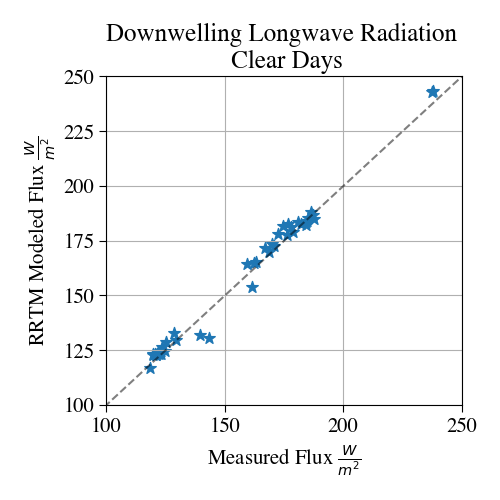
\includegraphics[width=0.65\linewidth]{figures/chapter4/RRTMcorrelation.png}
    \caption[RRTM modeled downward longwave flux vs measured flux.]{Modeled downward longwave flux as calculated by RRTM vs the observed downward LW flux measured by the Kipp and Zonen radiometers. The mean difference is 1.4 $W m^{-2}$ and the standard deviation is 3.6 $Wm^{-2}$. The maximum difference between the measurements and model results is 7 $Wm^{-2}$.}
    \label{fig:rrtm}
\end{figure}

\section{Results and Discussion}

Provide context for this section. Why are cloud macrophysical and radiative effects from N-ICE2015 important? 1) First, seasonal transition from winter to summer that has been measured since SHEBA, 2) unique winter storms were measured; extremely large and rapid transitions of cloud properties that coincide with changes in turbulent fluxes documented by \citet{walden:2017} and \citet{graham:2017}.

\subsection{Cloud Macrophysical Properties}

The upper panel of Figure \ref{fig:cloudmacro} shows the cloud fraction, or the percentage of the day that cloud was observed over the MPL, indicated by black squares. During the first half of the experiment in winter, it was common for days to have cloud fractions below 50 $\%$, with 16 out of the 61 days prior to the long break in observations having less than 50 $\%$ cloud cover. After the break, however, there are only 12 days out of the 89 days that are below 50 $\%$ cloud cover. The mean cloud fraction during the first half of the experiment is 70 $\%$ (standard deviation of 30 $\%$), and after is 75 $\%$ (standard deviation of 28 $\%$). Climatologically, a decrease in clear days has been seen for this region, contributing to a long-term warming trend \citep{kayser:2017}. The entire experiment, including a large number of cloudy days, is put into climatological context by \citet{graham:2017} and \citet{kayser:2017}. For the purpose of this study, there was significantly less cloud cover in winter than in the spring and summer.

\begin{figure}[H]
    \centering
    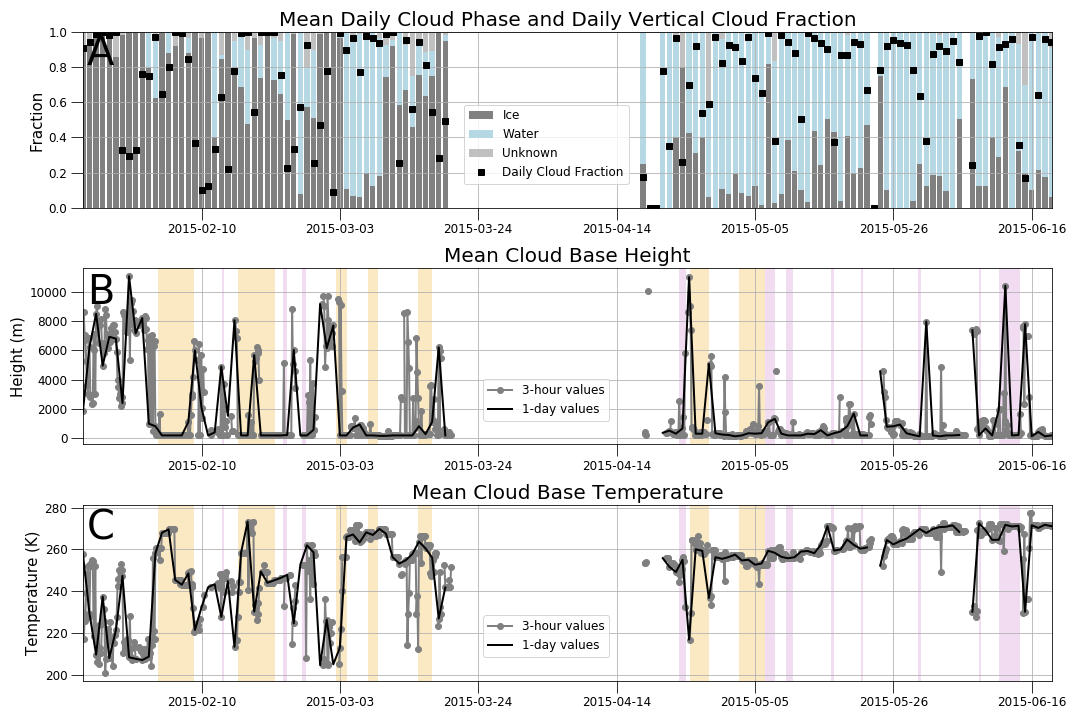
\includegraphics[width=1\linewidth]{figures/chapter4/ch2_f4.png}
    \caption[Cloud fraction/phase, height, and temperature.]{Top panel shows the mean daily cloud phase (the mean percentage of all clouds throughout the day that are water (blue), ice (dark gray), and unknown (light gray)). Daily cloud fraction is shown as black dots, showing what percent of the day the mean cloud phase represents. The middle panel shows both the 3-hourly (gray) and daily (black) mean cloud base height. Storm periods are shown in the middle and bottom panels in orange (major) and pink (minor) shading.}
    \label{fig:cloudmacro}
\end{figure}



During Floes 1 and 2 (winter), every day has at least some ice cloud present. Most of the days have primarily ice clouds with the exception of a week in early March, which corresponds to a period in which the cloud base was low and cloud temperature was near freezing (265-270 $K$). Some days have a small percentage of unknown cloud fraction, but this category only exceeds 20 $\%$ of the daily cloud existence once during the first half of the experiment. By visual inspection, these unknown clouds are primarily high, thin clouds that likely have little impact on the cloud radiative forcing at the surface.

The fraction of water clouds greatly increases during Floes 3 and 4 (spring and summer). These results are not surprising, as increasing temperature and increasing water fraction are expected. There are still ice clouds present on nearly every day through the end of the experiment, many of which are high, thin clouds. The water clouds, however, were primarily thick and close to the surface. Some of the ice can be attributed to mixed-phase clouds with both water and ice through the mid-troposphere, but low-level ice clouds were not common during the last two floes of the experiment.

Cloud base heights (Figure \ref{fig:cloudmacro}, middle panel) in the first month of the experiment are, on average, higher than the rest of the experiment. Once Floe 3 starts cloud base heights are almost entirely below 2 $km$. Figure \ref{fig:crf_timeseries} shows the frequency of cloud base heights for each month throughout the experiment with lines indicating the mean cloud base height. The mean height for January is 6.45 $km$, while the rest of the months' mean cloud heights are below 2 $km$. Mean cloud heights decrease throughout the experiment, with the lowest mean cloud base height present in June at just below 1 $km$. During the second half of the experiment, the majority of the clouds have a low cloud base height and a high percentage of water present. These clouds had large enough optical depths that they caused complete attenuation of the micropulse lidar beam, resulting in an inability to view clouds above them. As mentioned above, this inhibits the ability to report on higher-level clouds but does not impact the ability to understand the surface energy budget.

\begin{figure}[H]
    \centering
    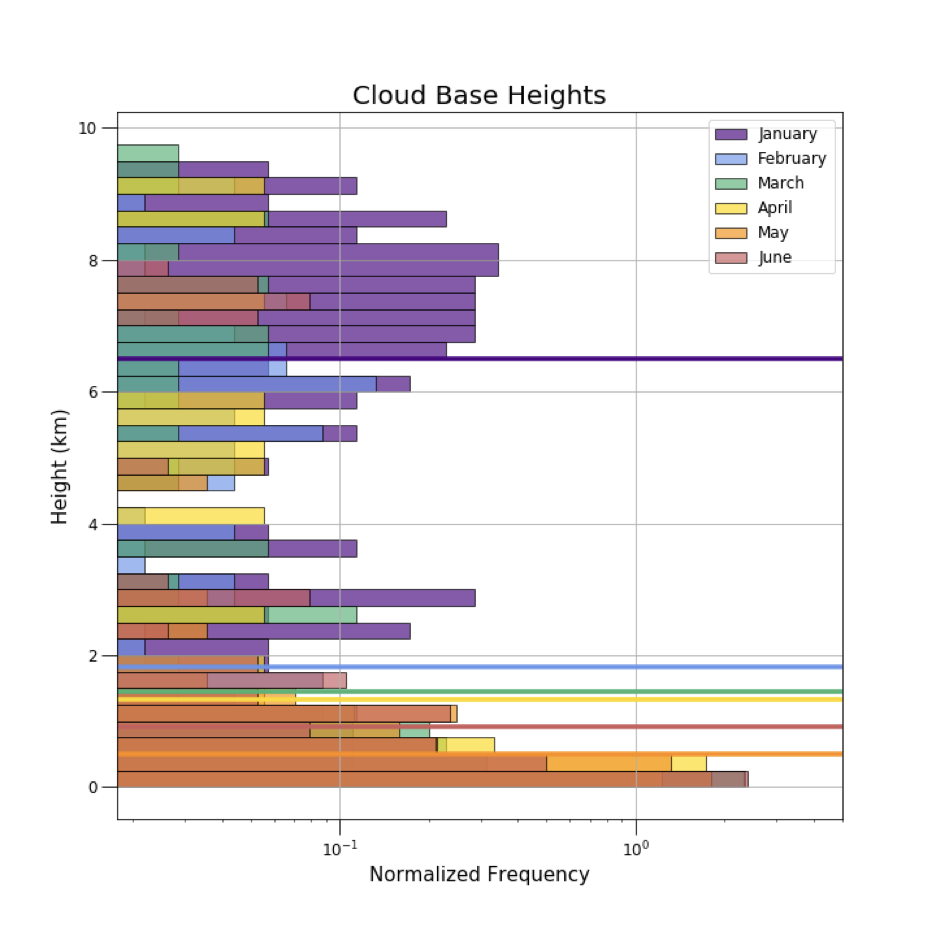
\includegraphics[width=0.75\linewidth]{figures/chapter4/ch2_f5.png}
    \caption[Cloud base height by month.]{Cloud base height by month. Frequency distribution is shown as bars colored by month. The monthly mean cloud height is shown by the horizontal line in the corresponding color.}
    \label{fig:cloudbase}
\end{figure}

Cloud base temperature closely mimics the cloud base height for the majority of the experiment. During the second two floes, the cloud base temperature gradually approaches freezing while the cloud base height stays fairly consistently near the surface. This slow increase in cloud base temperature reflects the increase in atmospheric temperature as more solar radiation reaches the Arctic. One interesting case occurred during the M2 storm when the cloud base temperature changed, but the cloud base height did not. During this period, the cloud base temperature drops while the cloud base height does not. This case is described more in-depth in section 4.4.

\subsection{Cloud Radiative Properties}

This section describes the variations in shortwave and longwave fluxes measured throughout N-ICE2015. These fluxes are used to calculate the shortwave, longwave and net cloud radiative forcing throughout the campaign as defined by Eq. XX above. These measurements are then categorized according to the cloud macrophysical properties described above.

Figure \ref{fig:flux:all} shows the time series of the shortwave (upper), longwave (middle), and net (lower) radiative fluxes. During Floe 1 in January and February, net flux (also, net longwave flux) dips to around -50 $W m^{-2}$ during non-storm periods (unshaded) and approaches 0 $W m^{-2}$ during storm periods (shaded). During major winter storms, downward longwave flux increases from between 100 and 150 $W m^{-2}$ to around 300 $W m^{-2}$, sometimes within only a few hours. Upward longwave flux mirrors these changes decreasing from -200 to -300 $W m^{-2}$. During non-storm periods, the upward flux is around -200 $W m^{-2}$ while the downward flux is just over +100 $W m^{-2}$, resulting in negative net flux. When the net flux approaches zero, as it does during storm periods, it indicates that clouds are relatively low and warm and has a large enough optical thickness to balance the longwave flux coming from the surface.

\begin{figure}[H]
    \centering
    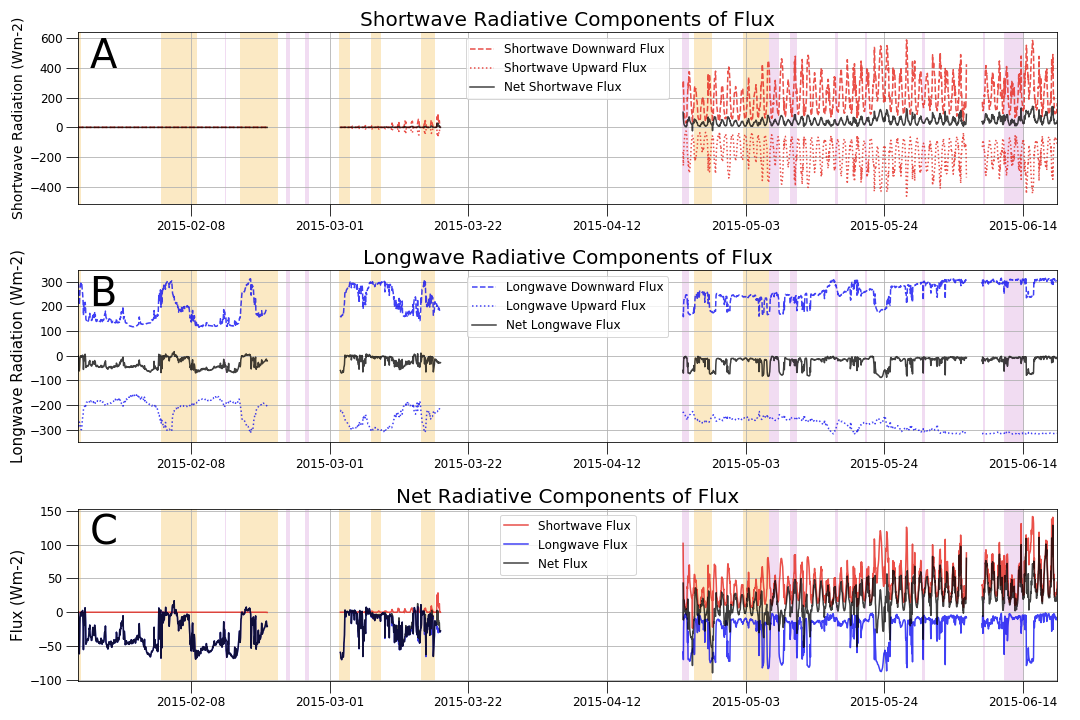
\includegraphics[width=1\linewidth]{figures/chapter4/ch2_f3.png}
    \caption[Shortwave, longwave, and net radiative components of flux.]{Shortwave (A), longwave (B), and net (C) components of radiative flux. Black lines represent net flux, dotted upward, and dashed downward. Major and minor storm periods are shown by the orange and pink shading, respectively.}
    \label{fig:flux:all}
\end{figure}

During Floe 2 in March, the downward and upward longwave fluxes more closely balance each other. This is due to a generally higher downward longwave flux from warmer cloud base temperatures and higher optical thicknesses from a greater fraction of liquid water clouds (Figure \ref{fig:cloudbase} C., discussed more thoroughly in the next section). During non-storm periods, the net longwave flux reaches a minimum just below -50 $W m^{-2}$, but is more frequently around -25 $W m^{-2}$. Storm periods continue to bring the net flux near 0 $W m^{-2}$, as lower and warmer clouds predominate. Small amounts of shortwave flux exist during the end of this floe as the sunlight returns to these latitudes (maximum of 50 $W m^{-2}$), but has little influence on net flux due to a large amount of reflected shortwave flux from the surrounding snow.

During Floe 3 in spring, the net longwave flux reaches as low as -70 $W m^{-2}$ but is often around 0 $W m^{-2}$. This is the result of increased and consistently high downward longwave flux. This is when the atmosphere is in an opaquely cloudy state \citep{stramler:, graham:2017}. As the experiment transitioned from winter into spring, cloud base height decreased and cloud occurrence increased. The decrease in cloud height and warming of the atmosphere results in an increased downward longwave flux from the clouds. In addition, during this period, the floe drifted into warmer ocean water \citep{kayser:2017} and the net shortwave flux increased, which increased the atmospheric temperature above the ice and the magnitude of the upward longwave flux. Upward longwave radiation is fairly consistent throughout this floe, starting around -225 to -250 $W m^{-2}$ in late April and steadily decreasing to around -300 $W m^{-2}$ in June. During this period, the upward longwave flux does not mirror the downward longwave flux as closely as it does during winter.

The net shortwave flux during Floe 3 generally fluctuates between 0 and 100 $W m^{-2}$, with only 6 days exceeding 100 $W m^{-2}$. The total net flux follows the daily pattern of the net shortwave flux and is primarily greater than 0 $W m^{-2}$. During the start of this floe, net flux drops below 0 $W m^{-2}$ during the two major storm periods. These drops are caused by both a decrease in net shortwave flux (due to increased cloud optical thickness) and a decrease in net longwave flux (higher cloud base and lower cloud base temperature, Figure \ref{fig:cloudbase} B and C). After this, there are a few more occurrences in which the flux decreases below 0 $W m^{-2}$, which coincide with decreases in the net longwave radiation, indicating higher cloud bases and/or lower cloud fractions (Figure \ref{fig:cloudbase}).  

Floe 4 in June experienced the greatest magnitude of net flux. Only two days (23 May and 15 June) had a daily average flux larger than 350 $W m^{-2}$. These days had primarily clear sky conditions. During the only storm period, net longwave flux decreases significantly (from around 75 $W m^{-2}$ to less than 50 $W m^{-2}$) due to a decrease in downward shortwave flux. This occurs at the same time as an increase in cloud base height from near the surface to around 10 $km$ (Figure \ref{fig:cloudbase} B). This is the largest decrease in flux during this floe. During this time, optically thick clouds block shortwave radiation from reaching the surface. However, because these cloud bases were warm and close to the surface, longwave flux rose to around 0 $W m^{-2}$ during this time, keeping net flux above 0 $W m^{-2}$. After the storm, net flux again drops to around the same magnitude as during the storm period, but this time accompanied by a decrease in downward longwave flux. This corresponds to an increase in cloud base height, a decrease in cloud base temperature, and a decrease in the cloud fraction (Figure \ref{fig:cloudbase}) indicating that, after the storm passed, clouds became high and more scattered, including a day with the lowest cloud fraction during this floe. 

Cloud radiative forcing at the surface (referred to as CRF) is shown in Figure \ref{fig:crf_timeseries}. (Here CRF is defined to be positive if there is net energy gained \emph{into} the surface.) Longwave CRF dominates the CRF throughout the field campaign. During Floes 3 and 4, the shortwave CRF has an increasing influence on the net CRF, but only decreases it by a small amount. Upward and downward shortwave CRF counteracts each other due to the high albedo of the snow cover on the sea ice, resulting in net shortwave CRF between -50 and 0 $W m^{-2}$. (\citet{walden:2017} report values of the surface albedo during N-ICE2015.) It is important to note that the clear-sky modeled radiation was estimated to be slightly less than the measured radiation, resulting in clear-sky periods to be slightly negative. This can be seen in the first floe when the upward longwave CRF is slightly below zero, creating a negative CRF. This does not mean that clouds were cooling the surface at this time. 

Because the CRF is positive throughout almost the entire field campaign, this indicates that clouds are generally warming the surface. During SHEBA and other studies \citep{schweiger:2004, cogley:1984, walsh:1998, curry:1996} clouds were found to warm the surface throughout the entire year except in mid-summer when the solar zenith angle was highest. The length of this cooling period was highly dependent on their albedo estimations \citep{intrieri:2002}. As N-ICE did not continue through the entire summer, it is impossible to say if there would be a period of negative cloud radiative forcing later in the summer in this region. But it is true that the CRF (net cloud radiative forcing) decreased with increasing solar radiation near the end of the campaign.

\begin{figure}[H]
    \centering
    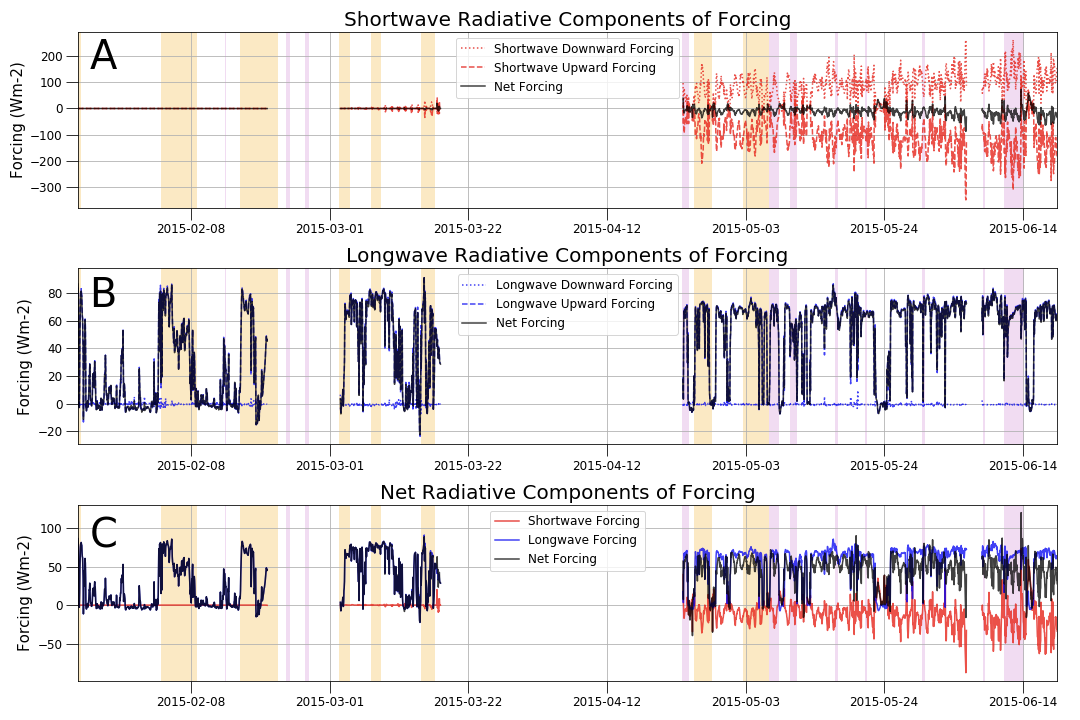
\includegraphics[width=1\linewidth]{figures/chapter4/ch2_f6.png}
    \caption[Shortwave, longwave, and net components of cloud radiative forcing.]{The same as Figure \ref{fig:flux:all} for the components of cloud radiative forcing.}
    \label{fig:crf_timeseries}
\end{figure}


\begin{figure}[H]
    \centering
    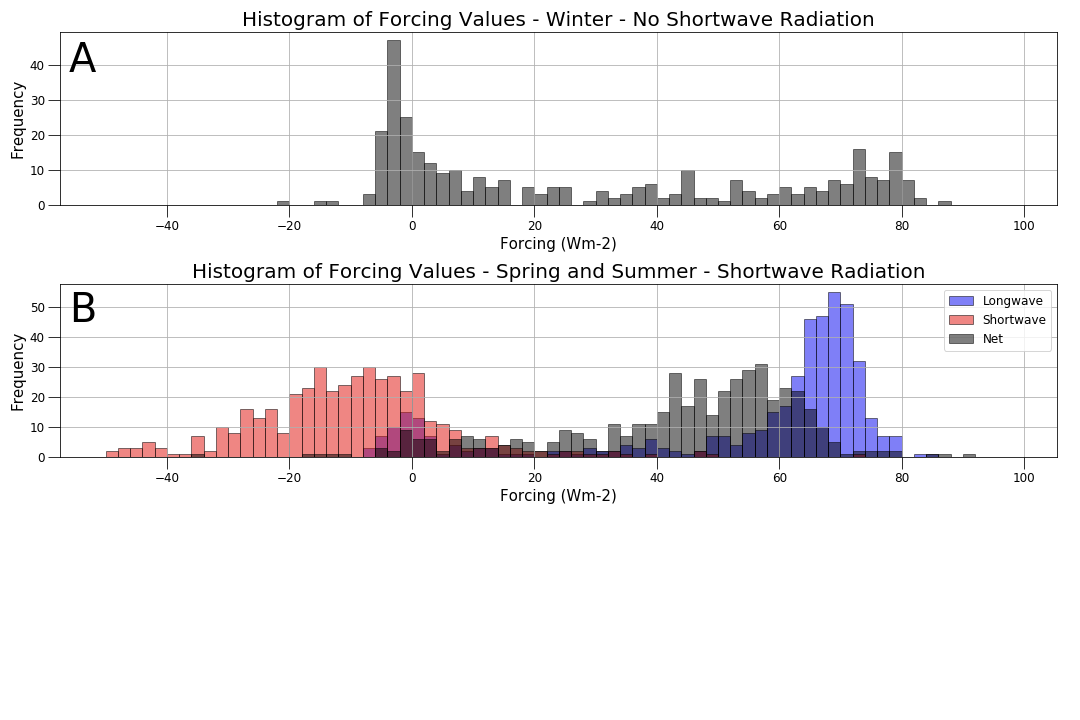
\includegraphics[width=1\linewidth]{figures/chapter4/ch2_f7.png}
    \caption[Histograms of cloud radiative forcing by season]{Histograms of cloud radiative forcing divided by season. Winter, when no shortwave radiation is present, is shown in the top panel. The longwave CRF and net CRF are the same at this time, so only the net CRF histogram is shown. Spring and summer (all times when there is shortwave radiation, labeled summer) are shown in the bottom histogram. Distributions are for longwave (blue), shortwave (red), and net (black) CRF.}
    \label{fig:crf_histo}
\end{figure}

Histograms of the longwave, shortwave, and net CRF, shown in Figure \ref{fig:crf_histo}, are divided by season depending on the presence of solar radiation. In winter (top panel), the histogram (longwave radiation only) shows a slightly bimodal distribution, with one large peak near 0 $W m^{-2}$ and another small peak between about 50 and 80 $W m^{-2}$. (Note that the negative value of the large peak at 3 $W m^{-2}$ may be due to the slight overestimation in the clear-sky flux.) These two modes describe clear (0 $W m^{-2}$ and cloudy (75 $W m^{-2}$) conditions. A range of cloud radiative forcing values up to the peak of about 85 $W m^{-2}$ is due to the range in cloud properties (fraction, phase) and their associated radiative impacts during the winter. The winter had quite variable cloud conditions compared to those in summer in terms of height, temperature, and daily fraction. The highest winter CRF, the peak in the histogram around 75 $W m^{-2}$, occurred during the storm periods when cloud fraction was large, clouds were primarily close to the surface and composed of ice, and the cloud base and surface temperatures both increased.  

In the summer (bottom panel), the range of net CRF is smaller relative to winter. This is due to the negative shortwave CRF (cooling) that counteracts some of the positive longwave CRF. Longwave CRF in summer is between about 0 $W m^{-2}$ and 80 $W m^{-2}$, with the latter peak being the larger of the two (unlike winter). The majority of clouds during summer result in from 50 to 80 $W m^{-2}$ of longwave CRF. Shortwave CRF is between about +10 to -30 $W m^{-2}$, with a few values as low as -40 $W m^{-2}$. The result of these two competing components of CRF is a slightly bimodal distribution with a small peak near 0 $W m^{-2}$ and a larger peak between 30 to 70 $W m^{-2}$. The peak near 0 $W m^{-2}$ is small due to the limited number of clear-sky days seen during the summer. Because clouds were consistently low and thick throughout the spring and summer, the net CRF was more uniform throughout these two seasons than in winter.

Figures \ref{fig:winter:crf} and \ref{fig:spring:crf} display how the net cloud radiative forcing depends on the cloud's macrophysical properties. Figure \ref{fig:winter:crf} is for winter (Floes 1 and 2), and Figure \ref{fig:spring:crf} is for spring and summer (Floes 3 and 4). During the winter, cloud base height, and cloud base temperature have the most effect on the net CRF. This is no surprise as the atmosphere is warmer close to the ground, resulting in low clouds having a larger longwave influence on the surface. \citet{shupe:2004} found that clouds with temperatures cooler than 243 $K$ (-30 $^{\circ}C$) often had similar longwave radiative properties to clear sky conditions. In winter during N-ICE, there is a transition in radiative values at around 235 $K$. Winter clouds with base heights greater than 235 K had a larger spread in cloud radiative forcing values of about 60 $W m^{-2}$. Values lower than this still had variation in CRF, but were within 20 $W m^{-2}$ of clear-sky conditions and were more sensitive to changes in cloud base temperature. In the summer, this transition occurred closer to the 243 $K$ cutoff reported by \citet{shupe:2004}. However, due to the limited number of high, cold clouds, there were not many clouds below this threshold. In summer, in the longwave, the CRF was close to zero for these lower temperatures, in better agreement with the results from \citet{shupe:2004}. 

Daily mean cloud fraction does not have as clear of a correlation with daily mean surface CRF; days with below 50 $\%$ cloud fraction have less than 10 $W m^{-2}$ of CRF, while days with cloud fraction greater than 50 $\%$ can have CRF values that range from around 0 to just under 80 $W m^{-2}$. These slight trends were also seen by \citet{shupe:2004} during the SHEBA experiment. 

In spring and summer, the relationships between cloud base height and cloud base temperature are less obvious. This is due to the lack of variety in cloud characteristics during this period and the dependence on solar zenith angle. Most clouds were below 2 $km$ with cloud base temperatures above 250 $K$. Periods of higher, cooler clouds were present only during a few storm periods, one near the end of the experiment. These clouds had a higher ice fraction than the other summer clouds, likely due to their height. Cloud properties (such as height, phase, and temperature) have a large influence on longwave.

There is no apparent correlation between the fraction of cloud that is water and the amount of CRF in either season. \citet{schweiger:1999} started that the relationship between particle size and the amount of longwave CRF is not significantly different for liquid and ice particles. There is a significant difference, however, in shortwave CRF, as the different shapes have different influences on shortwave scattering. However, results from N-ICE do not show differences in water and ice clouds. This is likely due to the inability to determine the thickness of the cloud, as the lidar pulse will attenuate near the base of optically thick clouds, and the wide variety of solar zenith angles that were experienced during the transition to summer. 

\begin{figure}[H]
    \centering
    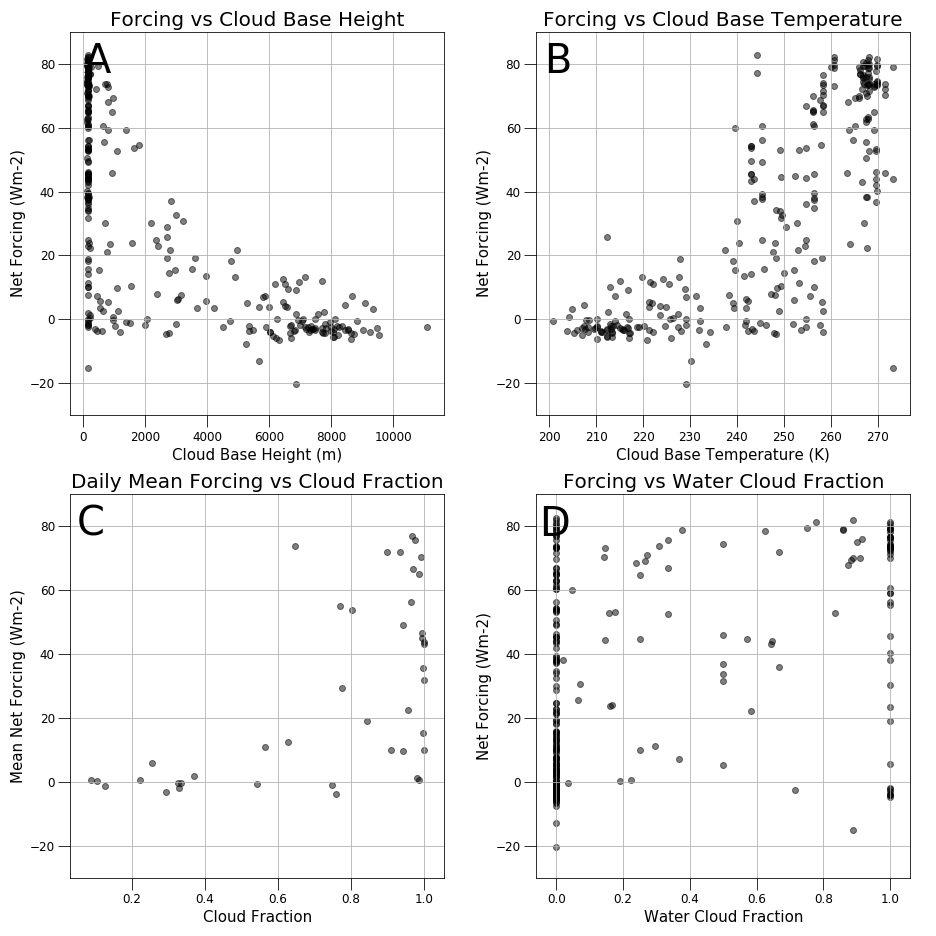
\includegraphics[width=1\linewidth]{figures/chapter4/ch2_f8.png}
    \caption[Cloud radiative forcing vs cloud base height, cloud base temperature, cloud fraction, and water cloud fraction]{Cloud radiative forcing vs cloud base height (A), cloud base temperature (B), daily mean cloud fraction (C), and water cloud fraction (D) for the winter season (defined as the period when no shortwave radiation is present). Net cloud radiative forcing is only comprised of longwave radiation during this time of year, so black dots represent both the net longwave CRF and the net CRF.}
    \label{fig:winter:crf}
\end{figure}

\begin{figure}[H]
    \centering
    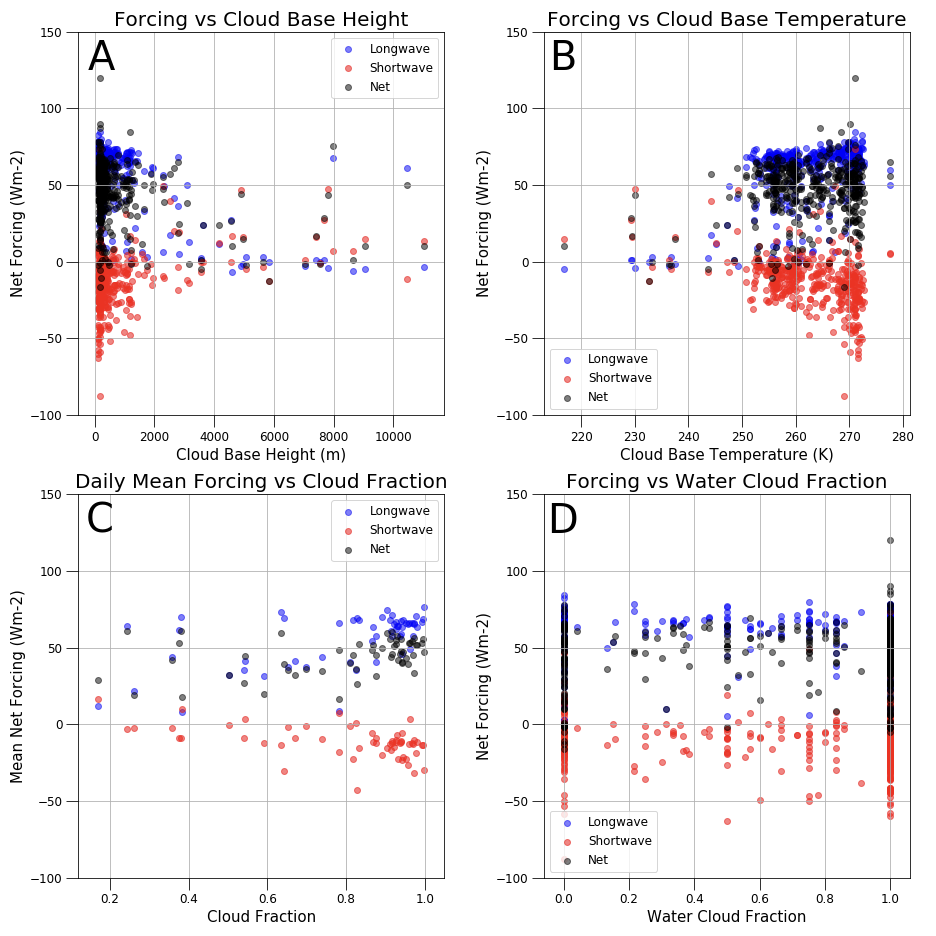
\includegraphics[width=1\linewidth]{figures/chapter4/ch2_f9.png}
    \caption[Spring and summer cloud radiative forcing vs cloud base height, cloud base temperature, cloud fraction, and water cloud fraction]{The same as Figure \ref{fig:winter:crf} for the spring and summer seasons. For these figures, spring and summer are defined as beginning when the shortwave radiation was no longer zero. This season has both longwave and shortwave radiation, shown in blue and red, respectively. Net radiation is shown in black.}
    \label{fig:spring:crf}
\end{figure}

\subsection{Cloud Effects during Winter Storms}

The longest storm period observed during N-ICE was the M2 storm, which took place from 3 February at 11:00 to 8 February at 21:00. This storm produced the most snowfall throughout the experiment (20.3 $mm$ of water equivalent) \citep{cohen:2017}. During this storm, a peak wind speed of 22 $m s^{-1}$ was reached, pressure decreased by 14 $hPa$ over a 6-hour period, and temperatures rose from -35.5 $^{\circ}C$ to -1.4 $^{\circ}C$. This storm, along with all other winter storms, was synoptically driven \citep{cohen:2017}. \citet{cohen:2017, walden:2017}, and Kayser et al. \citep{kayser:2017} detail the atmospheric conditions of storms and the period leading up to them throughout N-ICE. Figure \ref{fig:flux} shows the longwave components of flux and the components of cloud radiative forcing. (This storm took place in the winter, so there is no shortwave radiation to analyze.)

Net longwave flux is around zero throughout the storm period with the exception of the last day, when the downward longwave flux decreases while the upward flux stays the same, creating a negative net flux of about 50 $W m^{-2}$. During this storm period, CRF is between about 60 to 80 $W m^{-2}$ until just after the 5 February. After 5 February, net cloud radiative forcing decreases to between 30 to 60 $W m^{-2}$. This change in cloud radiative forcing corresponds to a decrease in both the upward and downward longwave flux, resulting in no change in the net flux. This change in CRF is the result of a cold front accompanied by a wind shift from southwest to northwest \citep{kayser:2017}. Figure \ref{fig:clouds} A shows the cloud fraction and the percentage of each phase within the clouds. During this decrease in CRF, there is more consistent cloud cover. A strong surface inversion of about 20 $^{\circ}C$ develops, resulting in a cooler surface and cooler conditions aloft, causing a decrease in longwave radiation from both the surface and the clouds. 

At the beginning of 6 February, the cloud base temperature decreases without an increase in cloud base height (Figure \ref{fig:clouds} B), indicating that temperatures throughout the atmosphere dropped during this time period, possibly in response to the decreased cloud radiative forcing. At the end of the storm period, the temperature continues to decrease as cloud heights increase and CRF decreases. During this time, the cloud fraction decreases, indicating that, as the storm dissipates, the sky begins to clear and cool the surface. 

\begin{figure}[H]
    \centering
    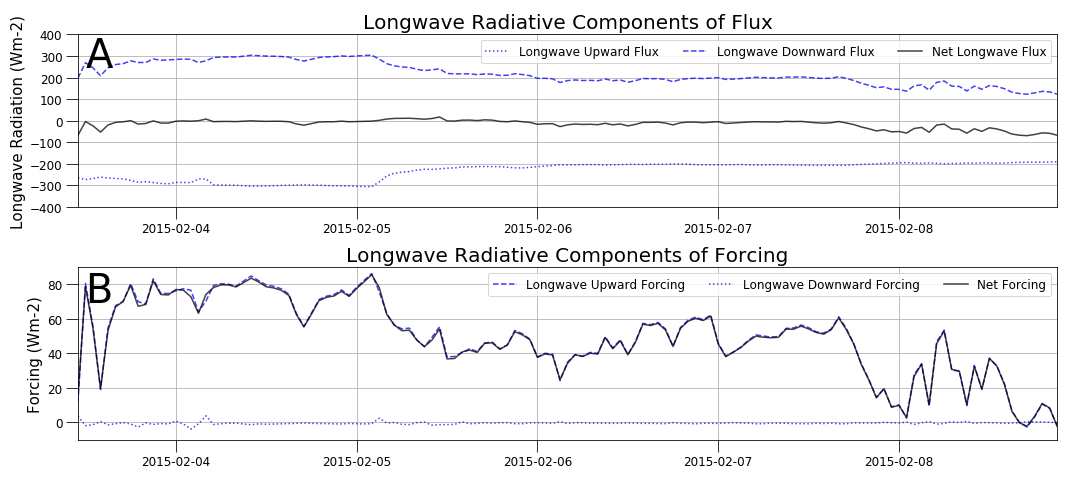
\includegraphics[width=1\linewidth]{figures/chapter4/ch2_f10.png}
    \caption[Longwave radiative components of flux and cloud radiative forcing]{Longwave radiative components of surface flux (A) and longwave radiative components of cloud radiative forcing at the surface (B). Upward flux/CRF is in the dotted line, downward is in the dashed line, and net CRF is in the solid line. The bottom figure shows that the upward CRF dominates the net longwave CRF, so those two lines overlap.}
    \label{fig:flux}
\end{figure}

\begin{figure}[H]
    \centering
    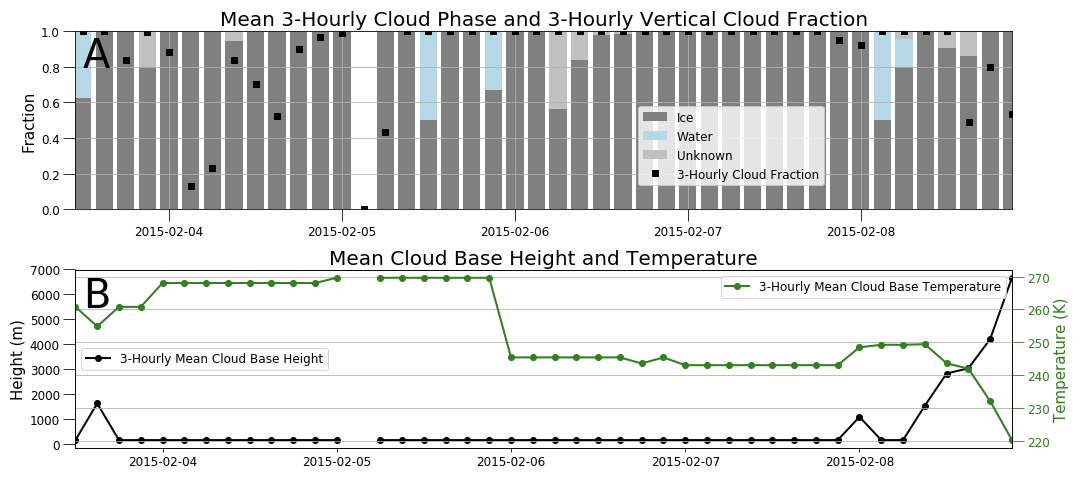
\includegraphics[width=1\linewidth]{figures/chapter4/ch2_f11.png}
    \caption[Cloud phase, fraction, base height, and base temperature.]{The top panel (A) shows the three-hourly fraction of cloud phase and vertical cloud fraction for the M2 storm period. The bottom panel (B) shows the 3-hourly mean cloud base height (black, left y-axis), and the 3-hourly mean cloud base temperature (green, right y-axis).}
    \label{fig:clouds}
\end{figure}

\section{Conclusions}